\documentclass[journal]{IEEEtran}

\usepackage{amsmath,amssymb}
\usepackage{graphicx}
\usepackage{booktabs}
\usepackage{array}
\usepackage{multirow}
\usepackage{cite}
\usepackage{url}
\usepackage[hidelinks]{hyperref}

\graphicspath{{figures/}}
\newcommand{\pstatic}{p_{\mathrm{s}}}
\newcommand{\pdynamic}{p_{\mathrm{d}}}
\newcommand{\pfused}{p_{\mathrm{f}}}
\newcommand{\xfull}{\textsc{XAI-Full}}

\title{A Multi-Stage Framework for PE Malware Detection:\\
Explanation-Guided Active Learning and Controlled XAI Fidelity Evaluation}

\author{Luu Van Doanh and Truong Ninh Thuan%
\thanks{The authors are with the VNU University of Engineering and Technology,
Vietnam National University, Hanoi, Vietnam.}%
}

\begin{document}

\maketitle

\begin{abstract}
Early malware detection must balance rapid decisions against behavioral evidence
that becomes available only after execution. Static classifiers are efficient but
remain exposed to packing, obfuscation, and distribution shift; dynamic analysis
can reveal intent but introduces observation delay and can be evaded by dormant
execution. A third operational difficulty is adaptation: expert labels are costly,
and explanations are often presented without testing whether they reflect model
behavior. This paper develops a multi-stage framework that connects three
mechanisms: a provenance-aware design for proportional--integral--derivative
(PID) fusion of static and dynamic scores; an explanation-guided active-learning
policy combining predictive uncertainty, TreeSHAP directional entropy, and SHAP
variance; and a controlled feature-space fidelity evaluation with equal-budget
random masking. In a verified row-disjoint pilot of 2,000 feature vectors with
unverified upstream sample provenance, the full acquisition policy achieved a
mean ROC--AUC of $0.9749\pm0.0040$ at 700 training labels, compared with
$0.9691\pm0.0046$ for uncertainty sampling and $0.9634\pm0.0063$ for random
sampling. Its paired AUC advantage over uncertainty sampling was positive in all
five seeds, whereas false-positive-rate improvement occurred in only two. For a
separately fitted fidelity model, replacing the 25 largest absolute-SHAP
coordinates by training means reduced ROC--AUC from 0.9802 to 0.8185; 20 random
masks of equal size retained a mean ROC--AUC of 0.9799. The results support
explanation-guided prioritization and the behavioral relevance of the SHAP
ranking under the specified feature-space intervention. Because aligned real
dynamic observations are unavailable, PID effectiveness and end-to-end latency
remain open empirical questions rather than reported system results.
\end{abstract}

\begin{IEEEkeywords}
active learning, explainable artificial intelligence, explanation fidelity,
LightGBM, malware detection, PID fusion, portable executable, ransomware,
TreeSHAP
\end{IEEEkeywords}

\section{Introduction}
\label{sec:introduction}

Ransomware compresses the defender's decision window. A detector must identify a
malicious program early enough to prevent encryption and lateral impact, yet much
of the most discriminative evidence appears only after execution. Static analysis
can score a Windows portable executable (PE) before it runs and is therefore
attractive for low-latency screening. Modern static detectors learn from byte
distributions, header fields, imports, sections, strings, and related PE
attributes; tree ensembles remain strong tabular baselines on EMBER-style
representations \cite{anderson2018ember,harang2020sorel,ke2017lightgbm}. Their
speed, however, does not remove brittleness under packing, obfuscation, family or
temporal shift, and manipulation of non-functional PE content
\cite{ucci2019survey,gibert2020rise,arp2022dos}.

Dynamic analysis observes execution through file-system, process, registry,
memory, and network events. It can reveal destructive intent that a static
representation conceals and is especially relevant to ransomware, whose impact
is expressed through sequences of discovery, access, modification, and
encryption \cite{alrimy2018survey,kharraz2015cutting,bacci2021ransomware}.
Dynamic evidence nevertheless has its own failure modes. It costs time and
compute, its coverage depends on the analysis environment, and environment-aware
or sleep-delayed malware may withhold behavior during the observation window
\cite{sgandurra2016automated,sikorski2012practical}. Hybrid detection is thus a
natural design choice, but an unqualified average assumes that the reliability of
static and dynamic scores is fixed. This is hard to justify when behavioral
evidence arrives sequentially and may change in informativeness across a session.

The static model also creates two operational problems. First, continuous
adaptation requires labels for emerging, obfuscated, or ambiguous samples.
Expert attention is limited, so the system should prioritize examples that are
informative for retraining rather than annotate an arbitrary stream. Classical
uncertainty sampling selects points close to the current decision boundary
\cite{settles2009active,cohn1996active}, but output ambiguity alone does not reveal
whether the model relies on internally conflicting or concentrated evidence.
Second, an explanation graphic is not proof that the identified features govern
the prediction. Attribution methods can be unstable, can be evaluated using
unrealistic perturbations, and can encourage causal interpretations unsupported
by a predictive model \cite{guidotti2018survey,yeh2019infidelity,
warnecke2020evaluating}. In malware analysis this concern is acute because PE
features are constrained and correlated: changing an isolated coordinate in a
vector need not correspond to any executable file.

This paper studies the intersection of those problems through a multi-stage
framework centered on a LightGBM static classifier and native TreeSHAP
attributions. The framework includes an uncertainty gate for allocating dynamic
analysis, a stateful PID rule for fusing aligned static and dynamic evidence, an
active-learning acquisition score derived from prediction and explanation
signals, and a controlled fidelity protocol. The work deliberately separates
three claims that are often blended: predictive performance, label-selection
quality, and explanation fidelity. Each requires different controls. Moreover,
the available artifact supports quantitative conclusions for active learning and
feature-space fidelity, but not for PID fusion, because it does not contain
independently observed dynamic scores aligned with the static samples. Treating
that absence as a result would turn a system design into an empirical claim.

We organize the investigation around three research questions:

\begin{itemize}
    \item \textbf{RQ1:} At a fixed training-label budget, does a query score that
    combines predictive uncertainty with signed TreeSHAP geometry improve ranking
    performance over random and uncertainty-only acquisition?
    \item \textbf{RQ2:} Under an explicitly defined feature-space intervention,
    does deleting the largest absolute TreeSHAP contributions change model
    behavior more than random deletion with the same coordinate budget?
    \item \textbf{RQ3:} What evidence and controls are required to determine
    whether stateful PID fusion improves over static-only, dynamic-only, fixed,
    and simpler P/PI rules without confusing fusion time with dynamic-analysis or
    end-to-end latency?
\end{itemize}

The principal contributions are as follows.

\begin{itemize}
    \item \textbf{A provenance-aware multi-stage specification.} We formulate a
    static--dynamic architecture and a discrete PID update whose state is reset at
    independent session boundaries. The evaluation protocol locks gains,
    thresholds, and fusion baselines on validation data, requires one-to-one
    evidence linkage, and distinguishes offline score replay from signal
    acquisition and end-to-end latency. This contribution is a falsifiable design;
    no PID performance value is reported without aligned real observations.

    \item \textbf{An explanation-guided acquisition policy with controlled
    ablations.} The query score combines normalized predictive uncertainty,
    directional entropy of positive versus negative TreeSHAP mass, and variance
    across signed feature contributions. Under identical initial sets, splits,
    budgets, and five paired seeds, the full policy reached
    $0.9749\pm0.0040$ ROC--AUC with 700 training labels. The AUC difference from
    uncertainty sampling was positive in all five seeds. We report AP, FPR, TPR,
    partial ablations, learning curves, and query-time scope rather than reducing
    the outcome to a single favorable metric.

    \item \textbf{A controlled fidelity assessment for PE feature vectors.}
    Native TreeSHAP additivity is checked on raw log-odds, selected coordinates
    are replaced by arithmetic means estimated only from the training partition,
    and top-$|\mathrm{SHAP}|$ deletion is compared with 20 uniform random masks at
    each budget. At $k=25$, the top-SHAP AUC drop was 0.1616, approximately 630
    times the mean random drop of 0.000257. Faithfulness, explanation consistency,
    and contrastive separation are reported separately because they have
    different scales and assumptions; an Overall Fidelity Score (OFS) is not
    constructed without a validated aggregation rule.

    \item \textbf{A replay-oriented evidence package.} The measured run records
    fixed splits, source hashes, 150 model checkpoints, query decisions,
    per-sample predictions, mask indices, and pre/post-mask scores. Independent
    verification replayed 120,000 active-learning predictions, 12,500 query
    records, 63 mask batches, and 25,200 fidelity predictions. This supports
    computational traceability while explicitly not claiming provenance that the
    source CSV does not provide.
\end{itemize}

The evaluation is intentionally described as a row-disjoint internal pilot. The
CSV contains 2,000 rows and 2,381 numeric coordinates, but the repository does
not establish the original PE identities, collection dates, malware families, or
whether every positive label specifically denotes ransomware. Consequently, the
paper does not call the experiment a SOREL-20M benchmark, a family-held-out
test, a temporal test, or a zero-day evaluation. These limits reduce the scope of
the conclusion, but they also make the evidence auditable and prevent an
attractive system narrative from outrunning its data.

The remainder of this paper is structured as follows. Section~\ref{sec:related}
positions the work relative to static/dynamic detection, active learning, and
security XAI. Section~\ref{sec:problem} defines the problem, threat model, and
claim boundaries. Section~\ref{sec:method} presents the architecture, PID
specification, acquisition policy, and fidelity measures. Sections~\ref{sec:exp}
and~\ref{sec:results} describe the reproducible protocol and measured outcomes.
Sections~\ref{sec:discussion} and~\ref{sec:threats} discuss implications and
validity threats, and Section~\ref{sec:conclusion} concludes the paper.

\section{Related Work}
\label{sec:related}

\subsection{Static PE Malware Detection}

Static malware analysis extracts evidence without executing the suspect object.
Traditional workflows combine signatures, disassembly, imported functions,
strings, and manually engineered indicators \cite{sikorski2012practical}. Machine
learning expanded that workflow by learning discriminative patterns from fixed
representations. Saxe and Berlin combined structural attributes with a neural
network \cite{saxe2015deep}, whereas Raff \emph{et al.} studied learning directly
from raw executable bytes \cite{raff2018malware}. Tree ensembles remain attractive
for structured PE data because they train efficiently and expose native feature
contribution mechanisms. LightGBM uses histogram-based learning and leaf-wise
tree growth to scale gradient boosting \cite{ke2017lightgbm}; it is the static
learner used in this work.

Public resources improved comparability. EMBER introduced a documented static PE
feature representation and benchmark data \cite{anderson2018ember}. SOREL-20M
increased the scale and supplied metadata and labels suitable for large-scale
experiments \cite{harang2020sorel}. Such benchmarks do not remove evaluation
pitfalls. Random row splits can overestimate operational generalization when
near-duplicates, collection sources, families, or time periods cross partitions.
Arp \emph{et al.} identify these and related methodological traps in security
machine learning \cite{arp2022dos}. Surveys likewise emphasize distribution
shift, adversarial manipulation, and the difference between laboratory accuracy
and deployed detection \cite{ucci2019survey,gibert2020rise}.

The present work uses the EMBER v2 dimensional schema only as a reference for
2,381 input coordinates. A matching dimension is insufficient to infer the
origin of the vectors. We therefore separate model reproducibility from dataset
provenance and restrict empirical claims to the audited CSV.

\subsection{Dynamic and Hybrid Ransomware Analysis}

Ransomware detection benefits from behavioral evidence because extortion and
encryption ultimately require interactions with host resources. Prior work has
modeled file operations, entropy changes, API calls, registry activity, process
behavior, and network events \cite{alrimy2018survey,kok2019ransomware,
bacci2021ransomware}. Kharraz \emph{et al.} analyzed ransomware behavior and
defensive opportunities beyond file signatures \cite{kharraz2015cutting}.
Dynamic-analysis systems such as EldeRan demonstrate that runtime features can
support early detection, while also exposing limitations of constrained
sandboxing \cite{sgandurra2016automated}.

Dynamic observation is not free. Execution must be initiated, monitored, and
terminated; event collection and feature construction incur latency; and malware
may detect virtualization, require user interaction, or delay its payload. A
hybrid detector can route ambiguous static cases to dynamic analysis, but two
questions remain. First, the gate must be evaluated for coverage: confident
static mistakes may never be escalated. Second, fusion should be compared with
simple baselines using the same paired signals. A stateful controller cannot be
credited for the benefit of merely adding an informative dynamic source.

PID controllers are foundational feedback mechanisms with well-understood
practical strengths and limitations \cite{astrom2001future}. Their application to
probability fusion is heuristic rather than a physical-control guarantee. A
discrete update may smooth or adapt weights across a meaningful sequence, but it
does not itself establish calibration, closed-loop stability, lower FPR, or lower
end-to-end latency. This paper therefore contributes an explicit validation
protocol and reserves performance claims until the required paired observations
exist.

\subsection{Active Learning for Security Data}

Pool-based active learning alternates between model fitting, acquisition from an
unlabeled pool, oracle annotation, and retraining. Uncertainty sampling is a
widely used baseline because it selects observations close to the model's current
decision boundary \cite{settles2009active}. Earlier statistical formulations also
view active learning as the selection of observations expected to reduce model
uncertainty or prediction error \cite{cohn1996active}. Alternative strategies use
committees, expected error reduction, representation diversity, density, or
combinations thereof.

Security data complicate this loop. Class imbalance affects both training and
operating-point metrics; campaign drift can invalidate a previously useful query
rule; and an adaptive adversary may influence which samples enter the pool
\cite{gama2014concept,arp2022dos}. Furthermore, predictive uncertainty is only one
kind of ignorance. Two samples can have the same output probability while their
evidence differs: one may have weak contributions throughout, while another may
contain large positive and negative attributions that cancel. The latter pattern
is relevant to obfuscated or hybrid-looking samples, but it is invisible to a
margin-only score.

Our acquisition function treats signed explanation geometry as an additional
signal. It does not assume that SHAP variance is posterior model uncertainty or
variance across an ensemble; it is explicitly the across-coordinate variance of
the signed TreeSHAP vector for one sample. The design is tested through partial
ablations (uncertainty plus entropy and uncertainty plus variance), a full
combination, random selection, and uncertainty-only selection under matched
budgets and initial sets.

\subsection{Explainable AI and Fidelity in Security}

Model-agnostic explanation methods such as LIME approximate a local decision
surface \cite{ribeiro2016why}. SHAP unifies additive feature attributions through
Shapley values \cite{lundberg2017unified}, and TreeSHAP enables exact or efficient
attribution for tree ensembles \cite{lundberg2020local}. These methods are useful
for inspecting models, but interpretability is not a single measurable property.
Faithfulness concerns whether highlighted inputs affect predictions; stability
concerns how explanations change under related inputs or model changes; and
contrastive structure concerns whether explanations distinguish cases of
interest. A method can perform well on one axis and poorly on another.

Evaluation research has exposed additional difficulties. Yeh \emph{et al.}
formalize infidelity and sensitivity \cite{yeh2019infidelity}; Hooker \emph{et al.}
show that feature-removal evaluation can itself induce distribution shift
\cite{hooker2019benchmark}; and Warnecke \emph{et al.} analyze explanation methods
in security settings where feature semantics and attacker manipulation matter
\cite{warnecke2020evaluating}. A zero replacement is particularly questionable
when zero is meaningful or far from the training distribution. Replacing a
coordinate with a training statistic is more defensible as a model-level
intervention, but still need not preserve a valid PE.

Table~\ref{tab:related-gap} summarizes the positioning. The contribution is not
the claim that uncertainty, SHAP, or masking is new in isolation. It is the
controlled connection among explanation-derived acquisition, paired ablations,
same-budget deletion controls, explicit replay verification, and a strict
separation between measured components and an unevaluated static--dynamic fusion
design.

\begin{table*}[t]
\centering
\caption{Representative literature and the evaluation gap addressed in this work. A check mark means that the cited work centrally evaluates the property; ``partial'' indicates a related but different scope.}
\label{tab:related-gap}
\scriptsize
\setlength{\tabcolsep}{3.5pt}
\begin{tabular}{p{2.2cm}p{2.9cm}*{5}{>{\centering\arraybackslash}p{1.5cm}}}
\toprule
Research line & Representative sources & Static PE & Dynamic & Active learning & XAI fidelity & Replay artifacts \\
\midrule
Static malware ML & \cite{saxe2015deep,raff2018malware,anderson2018ember,harang2020sorel} & \checkmark & -- & -- & -- & partial \\
Dynamic ransomware analysis & \cite{kharraz2015cutting,sgandurra2016automated,bacci2021ransomware} & partial & \checkmark & -- & -- & partial \\
Active learning & \cite{cohn1996active,settles2009active} & domain independent & -- & \checkmark & -- & method dependent \\
General XAI & \cite{ribeiro2016why,lundberg2017unified,lundberg2020local} & domain independent & domain independent & -- & partial & -- \\
Fidelity evaluation & \cite{yeh2019infidelity,hooker2019benchmark,warnecke2020evaluating} & partial & partial & -- & \checkmark & partial \\
This work & TreeSHAP-guided queries plus controlled deletion and a PID validation protocol & \checkmark & protocol & \checkmark & \checkmark & \checkmark \\
\bottomrule
\end{tabular}
\end{table*}

\section{Problem Formulation and Threat Model}
\label{sec:problem}

\subsection{Objects, Scores, and Decisions}

Let $x\in\mathbb{R}^{d}$ denote a static PE feature vector with $d=2381$ in the
available pilot. A static classifier $f_{\mathrm{s}}$ produces a bounded score
$\pstatic=f_{\mathrm{s}}(x)\in[0,1]$. The implementation uses this score as a
probability-like output, but the fusion design does not assume perfect
calibration. If dynamic analysis is invoked, an independently specified mapping
$f_{\mathrm{d}}$ converts observed behavior $z$ into a bounded dynamic score
$\pdynamic=f_{\mathrm{d}}(z)\in[0,1]$. The meaning of $\pdynamic$---calibrated
probability or risk score---must be fixed before evaluation.

The architecture contains a conceptual uncertainty gate $g(\pstatic)$. A common
deployment form uses two validation-selected thresholds $\tau_{\mathrm{low}}$ and
$\tau_{\mathrm{high}}$: scores outside the interval can receive an early static
decision, while scores inside it are escalated for behavioral observation. The
present measured artifacts do not evaluate this gate or its coverage. In
particular, they do not establish how often a confident static error would bypass
dynamic analysis. The fusion protocol instead evaluates all supplied, aligned
static--dynamic pairs; any future gate study must report both conditional quality
and the fraction of traffic escalated.

For each evaluated score $p$, a threshold $t$ maps the score to
$\widehat{y}=\mathbb{1}[p\geq t]$. Thresholds are selected on the validation
partition for a target true-positive rate (TPR) of 0.95 and are then frozen for
test evaluation. The test TPR is still reported because a validation target does
not ensure exactly the same operating point on test. With true positives (TP),
false positives (FP), true negatives (TN), and false negatives (FN),
\begin{equation}
\mathrm{TPR}=\frac{\mathrm{TP}}{\mathrm{TP}+\mathrm{FN}},\qquad
\mathrm{FPR}=\frac{\mathrm{FP}}{\mathrm{FP}+\mathrm{TN}}.
\label{eq:tpr-fpr}
\end{equation}
ROC--AUC and average precision (AP) summarize ranking, while FPR and TPR describe
the selected operating point \cite{fawcett2006roc,saito2015precision}.

\subsection{Active-Learning Setting}

Let $\mathcal{L}_r$ and $\mathcal{U}_r$ be the labeled and unlabeled training
pools at round $r$. The model $f_r$ is fitted only on $\mathcal{L}_r$. An
acquisition function $Q_r(x)$ ranks $x\in\mathcal{U}_r$, and the top $b$ rows are
sent to an oracle. In the pilot, the oracle is simulated by revealing an existing
label only after selection. This permits controlled comparison of query policies;
it does not measure analyst disagreement, annotation time, or monetary cost.

All strategies within a seed share the same initial labeled set, training pool,
validation set, test set, and cumulative label budget. The test partition is not
used for querying, parameter selection, threshold selection, or stopping. The
primary estimand for RQ1 is the paired test-metric difference between acquisition
strategies at the same seed and budget. Because the five runs share one test set,
seed variability describes sensitivity to initialization and queried samples, not
a population confidence interval over independently drawn test sets.

\subsection{Explanation Object and Intervention}

For a fitted tree model and input $x_i$, let
$\boldsymbol{\phi}_i=(\phi_{i1},\ldots,\phi_{id})$ be the signed TreeSHAP
contribution vector, excluding the bias term. Native TreeSHAP operates on the raw
log-odds scale and must satisfy the additive reconstruction
\begin{equation}
f_{\mathrm{raw}}(x_i)=\phi_{i0}+\sum_{j=1}^{d}\phi_{ij}
\label{eq:additivity}
\end{equation}
within numerical tolerance. This identity verifies the computation, not the
semantic correctness of an explanation.

To test model sensitivity, a mask $M_i^{(k)}$ selects $k$ coordinates for sample
$i$. The intervention replaces each selected value by the corresponding
arithmetic mean $\mu_j$ estimated from the training partition:
\begin{equation}
\widetilde{x}_{ij}=\begin{cases}
\mu_j, & j\in M_i^{(k)},\\
x_{ij}, & \text{otherwise}.
\end{cases}
\label{eq:mask}
\end{equation}
The top-SHAP mask contains the $k$ largest $|\phi_{ij}|$ values for each sample.
The control selects $k$ distinct coordinates uniformly at random. This is a
feature-space deletion test. It does not claim that $\widetilde{x}_i$ is produced
by a valid PE or a semantics-preserving binary edit.

\subsection{Threat Model and Scope}

The motivating adversary distributes Windows PE malware and may employ packing,
obfuscation, benign-looking metadata, delayed execution, intermittent activity,
or environment checks. Such behavior can weaken either evidence source: static
features may hide functionality, while a sandbox may not observe the payload
within its window. The current design does not claim robustness to a fully
adaptive attacker with white-box access to the static model, query function, and
fusion rule. Adversarial feature manipulation, explanation manipulation, and
active-learning poisoning remain outside the measured scope.

The defender is assumed to have a static feature extractor, a LightGBM model, an
optional isolated execution environment, and an oracle capable of assigning
labels to selected samples. A valid PID evaluation additionally assumes that
static and dynamic scores are aligned to the same sample and observation session,
that sequence order is meaningful, and that validation and test sessions do not
share controller state. These assumptions are enforced structurally by the
runner but cannot be satisfied by inventing $\pdynamic$ from the class label,
perturbing $\pstatic$ with random noise, or replaying an untraceable demonstration
log.

Finally, the empirical scope is narrower than the motivating threat model. The
audited CSV has binary labels but no verified original file identities, family
metadata, timestamps, or ransomware-specific label definition. We therefore use
``positive'' and ``negative'' when discussing measured classes. Ransomware is the
system motivation and intended deployment domain, not a provenance claim about
every evaluated row.

\section{Proposed Methodology}
\label{sec:method}

\subsection{Multi-Stage Architecture}

Figure~\ref{fig:architecture} separates the online decision path from the
offline adaptation and verification paths. The static path extracts a fixed PE
representation and applies LightGBM. A deployment gate may accept an early
decision or request behavioral observation. Once both scores are available, a
fusion rule returns a final score. TreeSHAP serves two distinct offline roles:
it contributes signals to active-learning acquisition, and it supplies
attributions for a controlled fidelity evaluation. The same explanation method
is used, but the estimands differ: acquisition asks which sample to label next;
fidelity asks whether a ranked set of coordinates affects the fitted model.

\begin{figure*}[t]
\centering
\fbox{\begin{minipage}{0.96\textwidth}
\centering
\textbf{Online evidence path}\par\medskip
PE sample $\rightarrow$ static feature vector $x$ $\rightarrow$ LightGBM
$\rightarrow \pstatic$ $\rightarrow$ uncertainty gate
$\rightarrow$ behavioral observation $z$ $\rightarrow \pdynamic$
$\rightarrow$ validated fusion rule $\rightarrow \pfused$ and decision
\par\medskip
\hrule
\medskip
\textbf{Offline adaptation and verification}\par\medskip
Unlabeled pool $\rightarrow$ TreeSHAP $\rightarrow$ $U,H,V$
$\rightarrow$ query ranking $\rightarrow$ oracle labels $\rightarrow$ retraining
\qquad$\mid$\qquad
Fixed model $\rightarrow$ top-$|\mathrm{SHAP}|$/random masks
$\rightarrow$ FF, EC, CF and replay verification
\end{minipage}}
\caption{Conceptual multi-stage framework. The verified pilot evaluates the
active-learning and fidelity branches. The gate and PID branch are specified but
require aligned real dynamic observations for empirical evaluation.}
\label{fig:architecture}
\end{figure*}

This separation prevents three timing quantities from being conflated. Static
inference time is the cost of the initial model; dynamic observation time includes
sandbox startup and the monitoring window; and fusion time is the arithmetic
replay after both scores exist. A fast fusion function cannot eliminate the time
needed to obtain $z$. Similarly, the time required to score an active-learning
pool does not measure annotation time.

\subsection{Static LightGBM and Native TreeSHAP}

LightGBM learns an additive ensemble of decision trees
\begin{equation}
F(x)=\sum_{m=1}^{M}\eta h_m(x),
\end{equation}
where $h_m$ is a tree, $M$ is the number of boosting rounds, and $\eta$ is the
learning rate \cite{ke2017lightgbm}. The binary score is obtained from the raw
logit through the logistic link. Tree models are appropriate for heterogeneous
PE feature groups and do not require the coordinates to share a unit or scale.

For a fitted booster, native TreeSHAP returns $d$ contributions and one bias
value. We verify (\ref{eq:additivity}) for every scored pool or fidelity sample.
The largest observed error was below $10^{-14}$ in both measured pipelines. All
rankings use the $d$ signed feature contributions; the bias is excluded. This
matters because including the bias as a feature would allocate the model's base
rate to the deletion budget and distort both acquisition and fidelity analyses.

\subsection{Adaptive PID Fusion Specification}

Suppose a session provides aligned pairs $(p_{\mathrm{s},k},p_{\mathrm{d},k})$ in a meaningful
order $k$. The implementation defines the discrepancy as
\begin{equation}
e_k=p_{\mathrm{s},k}-p_{\mathrm{d},k}.
\label{eq:pid-error}
\end{equation}
The state update is discrete by observation step:
\begin{align}
I_k &= I_{k-1}+e_k,\label{eq:pid-i}\\
D_k &= e_k-e_{k-1},\label{eq:pid-d}\\
u_k &= K_p e_k+K_i I_k+K_d D_k.\label{eq:pid-u}
\end{align}
The static weight is a clipped logistic transformation,
\begin{equation}
w_{\mathrm{s},k}=\operatorname{clip}
\left(\frac{1}{1+\exp(-u_k)},0.1,0.9\right),
\label{eq:pid-weight}
\end{equation}
and the fused score is
\begin{equation}
p_{\mathrm{f},k}=w_{\mathrm{s},k}p_{\mathrm{s},k}+
(1-w_{\mathrm{s},k})p_{\mathrm{d},k}.
\label{eq:fusion}
\end{equation}

The reference gains are $(K_p,K_i,K_d)=(0.85,0.12,0.35)$, but they are not
treated as established optima. The validation grid contains proportional gains
$\{0.425,0.85,1.7\}$, integral gains $\{0,0.06,0.12\}$, and derivative gains
$\{0,0.175,0.35\}$, together with simpler P and PI subsets. Fixed weights are
searched over $\{0,0.1,\ldots,1\}$. A candidate is selected by maximum validation
AUC, then lower validation FPR, then declared grid order. The decision threshold
is independently selected on validation for the target TPR.

The controller is reset for every independent \texttt{sequence\_id}, data split, seed,
and active-learning strategy. No state flows from validation into test. The
implementation contains neither an explicit $\Delta t$ nor integral anti-windup;
clipping the output weight is not the same as bounding the accumulated state. If
every sequence contains only one independent observation, the P, I, and D terms
cannot be interpreted as distinct historical benefits. A credible experiment
must therefore document why observations form a sequence and what one step
means.

Equations~(\ref{eq:pid-error})--(\ref{eq:fusion}) are a fusion heuristic, not a
stability theorem. When $\pstatic>\pdynamic$, the update tends to increase the
static weight; when $\pdynamic>\pstatic$, it tends to favor the dynamic score.
This often emphasizes the larger positive-risk estimate, but it does not
guarantee calibration or lower FPR. The required baselines are Static-only,
Dynamic-only, a 50/50 average, validation-selected fixed weighting, P, PI, PID,
and the untuned reference PID. The full design also includes a two-factor
comparison between Random/$\xfull$ querying and Fixed/PID fusion. A
difference-in-differences analysis is required before claiming interaction
between the two components.

\subsection{Explanation-Guided Active Learning}

At round $r$, the fitted model assigns probability $p_i$ to each pool sample.
Predictive uncertainty is
\begin{equation}
U_i=1-2|p_i-0.5|,
\label{eq:uncertainty}
\end{equation}
which equals one at the decision boundary and zero at the extremes. To represent
the directional structure of a signed SHAP vector, define the total positive and
negative attribution masses
\begin{equation}
A_i^+=\sum_j\max(\phi_{ij},0),\qquad
A_i^-=-\sum_j\min(\phi_{ij},0).
\end{equation}
When $A_i^++A_i^->0$, let
\begin{equation}
q_i=\frac{A_i^+}{A_i^++A_i^-}.
\end{equation}
Directional entropy is the binary entropy
\begin{equation}
H_i=-q_i\log_2 q_i-(1-q_i)\log_2(1-q_i),
\label{eq:entropy}
\end{equation}
with $H_i=0$ for a one-sided or zero attribution vector. $H_i$ is high when
large positive and negative contributions coexist. It is not the entropy of the
class probability distribution.

The third signal is signed SHAP variance across coordinates,
\begin{equation}
V_i=\frac{1}{d}\sum_{j=1}^{d}(\phi_{ij}-\bar{\phi}_i)^2,
\qquad
\bar{\phi}_i=\frac{1}{d}\sum_j\phi_{ij}.
\label{eq:variance}
\end{equation}
This quantity measures concentration/dispersion of one explanation. It is not
variance across trees, posterior samples, or independently trained models.

Because $U$, $H$, and $V$ occupy different numeric ranges, each signal is
min--max normalized over the current pool:
\begin{equation}
\widetilde{S}_i=\begin{cases}
\dfrac{S_i-S_{\min}}{S_{\max}-S_{\min}}, & S_{\max}>S_{\min},\\
0, & \text{otherwise}.
\end{cases}
\label{eq:normalize}
\end{equation}
The acquisition function is
\begin{equation}
Q_i=\alpha\widetilde{U}_i+\beta\widetilde{H}_i+
\gamma\widetilde{V}_i.
\label{eq:query}
\end{equation}
The complete policy uses $(\alpha,\beta,\gamma)=(0.3,0.4,0.3)$. Partial
ablations use $U+H=(3/7,4/7,0)$ and $U+V=(0.5,0,0.5)$; the uncertainty baseline
uses $(1,0,0)$. Random sampling assigns an independent random score. Ties are
resolved by ascending original CSV row identifier, making selection deterministic
given the score vector and seed.

One active-learning run follows six steps: (1) fit a fresh LightGBM model on the
current labeled set; (2) select a validation threshold; (3) evaluate and save
validation/test predictions; (4) compute $Q$ only for the remaining training
pool; (5) reveal labels for the top $b$ pool rows; and (6) repeat until the fixed
budget is exhausted. Test outcomes never affect queries or stopping. SHAP is
recomputed after each model update, so the acquisition geometry follows the
current classifier rather than a frozen initial explanation.

\subsection{Controlled Fidelity Measures}

The fidelity experiment fits a separate LightGBM model on the entire training
partition and computes TreeSHAP on the fixed test partition. For each $k$, it
compares the sample-specific top-$|\phi|$ mask in (\ref{eq:mask}) with 20 random
masks of the same selected-coordinate count. The model is not retrained after
masking; the experiment measures prediction sensitivity of one fitted model.

Let $p_i$ and $p_i^{(M)}$ denote original and masked probabilities. The raw
faithfulness statistic used by the thesis is
\begin{equation}
\mathrm{FF}_{\mathrm{raw}}=\frac{1}{n}\sum_{i=1}^{n}
\frac{|p_i-p_i^{(M)}|}{p_i+\epsilon},\qquad \epsilon=10^{-12}.
\label{eq:ff}
\end{equation}
It is intentionally unclipped and may exceed one when $p_i$ is small. We
therefore also report AUC before/after masking, paired AUC drop, and mean absolute
probability change. These quantities provide more interpretable context than an
isolated FF value.

Explanation consistency (EC) compares pairwise geometry. Standardize test
features with training means and standard deviations, compute the cosine
similarity matrix $C^x$, and compute the cosine similarity matrix $C^\phi$ of
signed SHAP vectors. EC is the Pearson correlation over the strict upper
triangles:
\begin{equation}
\mathrm{EC}=\operatorname{corr}
\left(\operatorname{ut}(C^x),\operatorname{ut}(C^\phi)\right).
\label{eq:ec}
\end{equation}
For $n=400$, this produces 79,800 pairs, but the pairs share samples and are not
independent observations for a naive significance test.

Contrastive fidelity (CF) describes separation of the two label-conditioned SHAP
centroids. With $\boldsymbol{c}_0$ and $\boldsymbol{c}_1$ denoting mean SHAP
vectors for the negative and positive test classes,
\begin{equation}
\mathrm{CF}=\frac{\|\boldsymbol{c}_1-\boldsymbol{c}_0\|_2}
{\max_i\|\boldsymbol{\phi}_i\|_2+\epsilon}.
\label{eq:cf}
\end{equation}
CF is a normalized geometric separation statistic. It is neither a causal metric
nor proof of explanation correctness. FF, EC, and CF use different scales and
constructs. Consequently, no OFS is reported; choosing normalization and weights
after observing results would manufacture a composite score without an empirical
meaning.

\subsection{Computational Considerations}

LightGBM prediction is proportional to the number and depth of traversed trees.
Native TreeSHAP adds pool-scoring overhead that grows with ensemble and path
complexity. The acquisition policy computes explanations only for methods that
use $H$ or $V$; uncertainty and random baselines avoid that cost. The fidelity
test requires one original prediction, one SHAP computation, three top-k masked
batches, and $3\times20$ random batches. Timing is reported only for the scope
actually measured and is not translated into endpoint latency or analyst cost.

\section{Experimental Methodology}
\label{sec:exp}

\subsection{Evidence Source and Data Audit}

All quantitative results in this paper come from the immutable review package
\texttt{results/measured\_20261014}. The run records source commit
\texttt{4bd07c6}, an empty working-tree status, and the input-CSV SHA-256 digest
\texttt{c733cc0c3e0950fa1d05d57d34c69d0a}\-
\texttt{034383e0c1a2fde0e6878b9e2e8c3668}. Hashes establish byte identity, not
factual provenance.

The table contains 2,000 rows, 2,381 feature columns, and one binary label. The
audit found no exact duplicate vectors. A deterministic stratified row split with
seed 42 assigned 60\% to the training/pool partition, 20\% to validation, and
20\% to test. Table~\ref{tab:data} reports the class counts. No original file hash,
collection time, family, source, or label-definition manifest is available. We
therefore do not claim that the positive class exclusively represents ransomware
or that the rows form a verified subset of SOREL-20M or EMBER.

\begin{table}[t]
\centering
\caption{Audited pilot partitions.}
\label{tab:data}
\small
\begin{tabular}{lrrr}
\toprule
Partition & Negative & Positive & Total \\
\midrule
Training/pool & 900 & 300 & 1,200 \\
Validation & 300 & 100 & 400 \\
Test & 300 & 100 & 400 \\
\midrule
Total & 1,500 & 500 & 2,000 \\
\bottomrule
\end{tabular}
\end{table}

The dimensional layout matches the EMBER v2 extractor reference. The groups in
Table~\ref{tab:feature-groups} describe an expected schema, not proof that the
CSV was generated from the documented extractor. Hashed imports, exports, and
section attributes can contain collisions; an individual coordinate need not map
to one human-readable API or semantic property.

\begin{table}[t]
\centering
\caption{Reference feature-group dimensions for a 2,381-coordinate EMBER v2 representation.}
\label{tab:feature-groups}
\small
\begin{tabular}{lr}
\toprule
Feature group & Dimensions \\
\midrule
Byte histogram & 256 \\
Byte-entropy histogram & 256 \\
String extractor & 104 \\
General file information & 10 \\
Header information & 62 \\
Section information & 255 \\
Imports & 1,280 \\
Exports & 128 \\
Data directories & 30 \\
\midrule
Total & 2,381 \\
\bottomrule
\end{tabular}
\end{table}

\subsection{Active-Learning Protocol}

We used five seeds: 11, 22, 33, 44, and 55. For each seed, stratified sampling
selected 200 initially labeled training rows; all five acquisition policies shared
that exact initial set and remaining pool. Each run completed five acquisition
rounds of 100 labels, producing budgets of 200, 300, 400, 500, 600, and 700
training labels. The 400 validation labels are additional and are not counted in
the training budget.

At every round and for every method, a new LightGBM booster was trained with 60
trees, learning rate 0.05, 15 leaves, maximum depth 4, and minimum 10 samples per
leaf. Feature and bagging fractions were one, and deterministic column-wise
training used two threads. Method-specific random, data, and feature seeds were
locked to the run seed. The compared strategies were Random, Uncertainty, $U+H$,
$U+V$, and $\xfull$ with weights specified in Section~\ref{sec:method}.

The threshold was selected from validation predictions to target TPR 0.95. We
then saved validation and test probabilities, predictions, labels, row IDs,
thresholds, and round budgets. For queried rows we saved rank, composite score,
raw $U/H/V$ signals, normalized signals, and revealed label. This enables both
selection replay and checks that no test or validation index enters training.

The primary ranking metrics were ROC--AUC and AP. Thresholded metrics were FPR
and TPR. We report mean and sample standard deviation across seeds, paired
within-seed differences, and normalized area under the learning curve (AULC)
computed by trapezoidal integration over the training-label budget. We do not use
five seed values as five independent test datasets. No target validation AUC was
predeclared, so the run does not estimate labels saved to a target. Query timing
includes pool prediction, TreeSHAP, additivity checking, and normalization; it
excludes labeling, training, sorting, and file I/O.

\begin{table}[t]
\centering
\caption{Core experimental configurations.}
\label{tab:configuration}
\small
\begin{tabular}{p{2.4cm}p{4.6cm}}
\toprule
Component & Configuration \\
\midrule
AL budgets & 200 initial; $5\times100$ queried; 700 final \\
AL seeds & 11, 22, 33, 44, 55 \\
AL model & 60 trees; depth 4; 15 leaves; $\eta=0.05$ \\
AL threshold & Validation-selected at target TPR 0.95 \\
Fidelity model & 100 trees; depth 4; 15 leaves; $\eta=0.1$; seed 42 \\
Fidelity masks & $k\in\{10,25,50\}$; 20 random controls per $k$ \\
Fidelity bootstrap & 500 stratified paired test resamples \\
Execution & Python 3.12.14; LightGBM 4.7.0; two threads \\
\bottomrule
\end{tabular}
\end{table}

\subsection{Fidelity Protocol}

The fidelity experiment trained a separate LightGBM classifier on all 1,200
training rows with 100 estimators, learning rate 0.1, 15 leaves, maximum depth 4,
minimum child size 20, random seed 42, and two threads. It evaluated all 400 test
rows. This model is not an active-learning final-round model; AUC values from the
two experiments must not be subtracted or interpreted as component-wise gains.

We computed native TreeSHAP contributions and checked raw-score additivity. For
each test sample and $k\in\{10,25,50\}$, the $k$ highest absolute contributions
were replaced using the training-column means. Twenty sample-specific uniform
random masks without replacement formed the control at each $k$. We recorded
the selected indices, number of coordinates that actually changed, original and
masked probabilities, AUC, AUC drop, signed and absolute probability changes,
and $\mathrm{FF}_{\mathrm{raw}}$. Random-control summaries report means and
sample SD across masks.

For uncertainty in the top-SHAP AUC drop, 500 stratified bootstrap resamples
preserved the original/masked prediction pair for each sampled test row. These
intervals are conditional on the one fitted model; they do not include
between-training variability. EC and CF were calculated once from the fixed test
explanations according to (\ref{eq:ec}) and (\ref{eq:cf}).

\subsection{PID Evaluation Protocol}

The default run intentionally did not execute fusion. A valid fusion input must
contain a dynamic score, \texttt{row\_id}, session identifier, sequence order, report
path, and SHA-256 digest for each observation. Metadata must declare the signal
as observed, document the score construction and collection policy, and confirm
that the score did not use the target label. Validation and test sessions must be
disjoint.

When such evidence becomes available, the runner joins each dynamic observation
to saved final-round active-learning probabilities. It tunes fixed, P, PI, and
PID rules only on validation, freezes the selected settings, evaluates on test,
and saves all fused predictions. Static-only, Dynamic-only, Average, and untuned
reference PID are included. The runner reports score-replay milliseconds per row
but labels this value as excluding collection, model inference, and I/O. No
fusion metric appears in Section~\ref{sec:results} because the required input is
absent.

\subsection{Independent Replay Verification}

The verification command reloads every active-learning checkpoint and
recomputes probabilities, metrics, and selected queries from saved row indices.
For fidelity, it reloads the model, training baseline, mask indices, and SHAP
inputs, reconstructs each masked matrix, and recomputes predictions and geometry.
The review package reports successful replay of 150 active-learning checkpoints,
120,000 active-learning prediction records, 12,500 query records, 63 mask
batches, and 25,200 masked prediction records. Verification establishes
computational consistency with the saved artifact; it cannot authenticate the
external origin of the CSV.

\section{Results}
\label{sec:results}

\subsection{RQ1: Active-Learning Performance}

Table~\ref{tab:al-final} reports final-round results at 700 training labels. The
complete explanation-guided policy obtained the highest mean ROC--AUC
($0.9749\pm0.0040$) and AP ($0.9442\pm0.0057$). Uncertainty sampling reached
$0.9691\pm0.0046$ AUC, while random selection reached
$0.9634\pm0.0063$. Thus, the mean final AUC differences were 0.0058 relative to
uncertainty and 0.0115 relative to random.

\begin{table*}[t]
\centering
\caption{Final active-learning results at an equal budget of 700 training labels. Values are mean $\pm$ sample SD over five paired seeds. The 400 validation labels are additional.}
\label{tab:al-final}
\small
\begin{tabular}{lcccc}
\toprule
Strategy & ROC--AUC & AP & FPR (\%) & TPR (\%) \\
\midrule
Random & $0.9634\pm0.0063$ & $0.9194\pm0.0115$ & $21.73\pm4.59$ & $93.80\pm2.28$ \\
Uncertainty & $0.9691\pm0.0046$ & $0.9363\pm0.0076$ & $19.87\pm4.65$ & $95.60\pm1.14$ \\
$U+H$ & $0.9676\pm0.0031$ & $0.9371\pm0.0015$ & $17.20\pm5.15$ & $93.00\pm2.35$ \\
$U+V$ & $0.9692\pm0.0062$ & $0.9392\pm0.0073$ & $28.33\pm7.23$ & $96.40\pm3.05$ \\
$\xfull$ & $\mathbf{0.9749\pm0.0040}$ & $\mathbf{0.9442\pm0.0057}$ & $17.53\pm4.85$ & $95.40\pm1.52$ \\
\bottomrule
\end{tabular}
\end{table*}

The paired result is more informative than the aggregate means. For every seed,
$\xfull$ exceeded Uncertainty in AUC. The differences for seeds
11, 22, 33, 44, and 55 were 0.0040, 0.0010, 0.0116, 0.0058, and 0.0065,
respectively. Their mean was $0.00579$ with sample SD $0.00390$. AP differences
were also positive for all five seeds, with mean $0.00792$. This consistency
supports the RQ1 conclusion that explanation-derived signals improved ranking
relative to uncertainty-only acquisition within the fixed pilot protocol.

The threshold metrics require a more cautious reading. Relative to Uncertainty,
the $\xfull$ FPR differences by seed were +1.67, +4.33, $-7.67$, +1.00, and
$-11.00$ percentage points, where negative favors $\xfull$. The method therefore
reduced FPR in only two of five seeds. Its mean FPR was lower by 2.33 points, but
the SD of the paired difference was 6.62 points. Test TPR also differed slightly
(mean difference $-0.20$ percentage points). We do not infer stable
false-positive reduction from the mean alone.

The partial ablations clarify why the full policy should not be reduced to one
signal. $U+H$ produced the lowest mean FPR in Table~\ref{tab:al-final}, but its
mean TPR was also the lowest and its AUC remained below the full policy. $U+V$
obtained AP comparable to the full policy but had the highest and most variable
FPR. Since thresholds were selected for a validation TPR target, these outcomes
illustrate operating-point transfer rather than a contradiction in AUC ranking.

Figure~\ref{fig:learning-curves} shows performance across all six budgets. The
normalized AUC AULC was $0.9614\pm0.0046$ for $\xfull$, compared with
$0.9547\pm0.0043$ for Uncertainty and $0.9470\pm0.0052$ for Random. AP AULC
showed the same ordering: 0.9222, 0.9133, and 0.8903, respectively. This indicates
that the final-round advantage was not created only at the last query batch.

\begin{figure}[t]
\centering
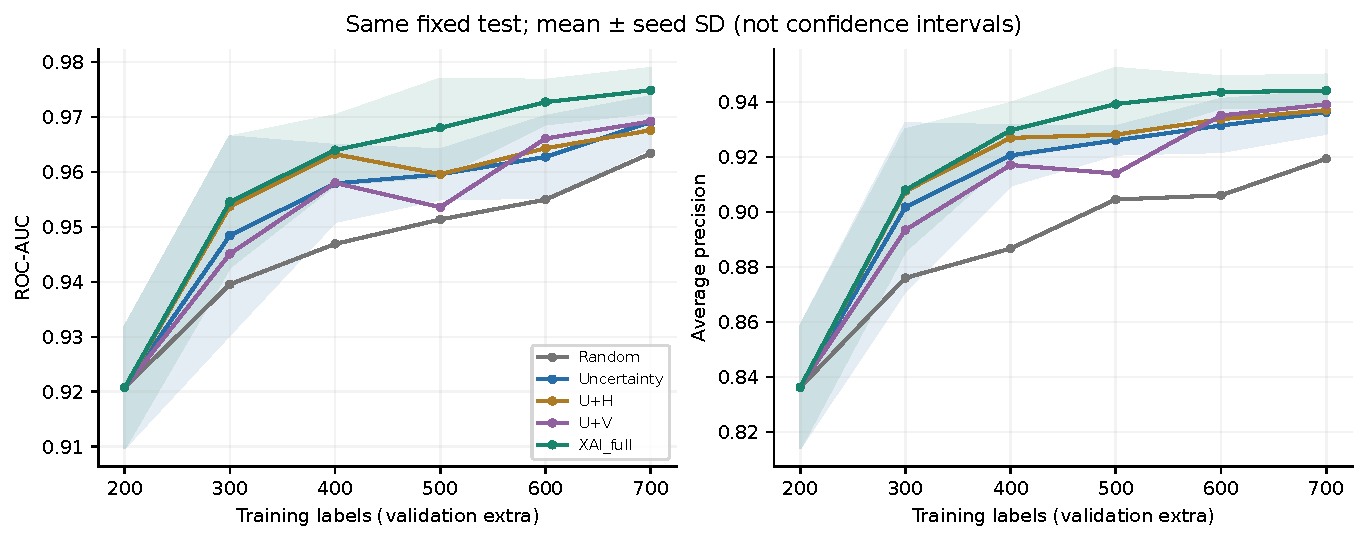
\includegraphics[width=\linewidth]{al_learning_curves.pdf}
\caption{Active-learning curves generated from the verified artifact. All methods
within a seed share the initial labeled set, split, and cumulative budget.}
\label{fig:learning-curves}
\end{figure}

\begin{figure}[t]
\centering
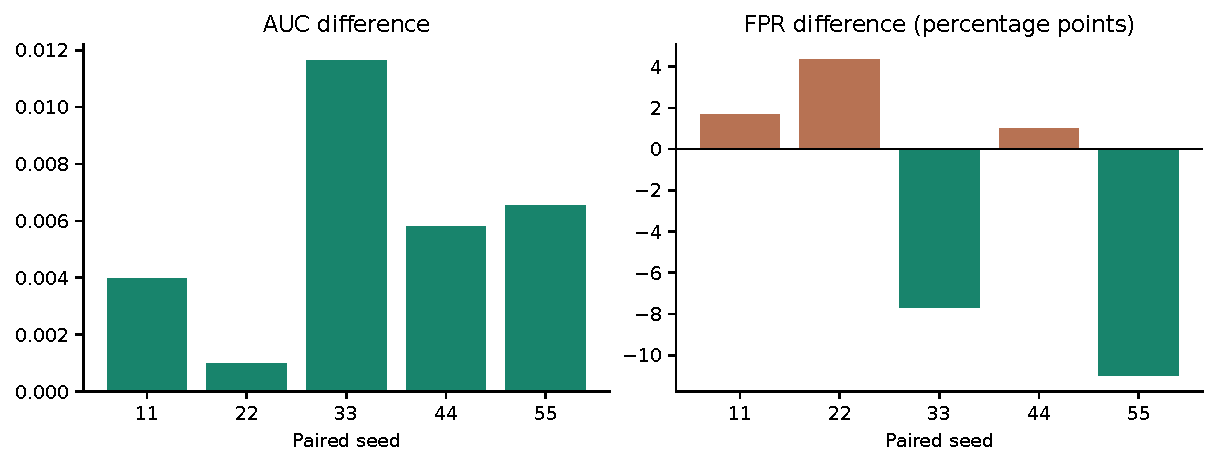
\includegraphics[width=\linewidth]{al_paired_differences.pdf}
\caption{Paired differences across seeds. AUC improvements are consistent for
$\xfull$ versus uncertainty, whereas FPR differences change sign.}
\label{fig:paired}
\end{figure}

Explanation-based acquisition incurred measurable scoring overhead. Mean total
query-scoring time across rounds was $0.1635$ s for $\xfull$, versus $0.0128$ s
for Uncertainty in the recorded two-thread environment. This approximately
13-fold ratio applies only to pool prediction, TreeSHAP, additivity checking, and
normalization in a small pilot. It excludes sorting, annotation, retraining, and
I/O and should not be interpreted as end-to-end operational latency.

The run trained 150 models: five seeds, five methods, and six budgets. The
maximum TreeSHAP additive reconstruction error in acquisition was
$4.44\times10^{-15}$. These checks reduce the likelihood that the observed
policy difference came from unequal initialization, accidental test access, or a
malformed attribution matrix. They do not resolve the external-validity limits of
the dataset.

\subsection{RQ2: Fidelity Under Controlled Deletion}

The separately fitted fidelity model obtained test ROC--AUC 0.980167 and AP
0.955338 before masking. Native TreeSHAP reconstructed the raw model score with
maximum absolute error $7.11\times10^{-15}$. Table~\ref{tab:fidelity} compares
sample-specific top-SHAP deletion with the mean across 20 equal-budget random
masks.

\begin{table*}[t]
\centering
\caption{Controlled feature-space deletion on one fixed model. Random AUC is the mean across 20 masks per $k$; bootstrap intervals condition on the fitted model.}
\label{tab:fidelity}
\scriptsize
\setlength{\tabcolsep}{3pt}
\begin{tabular}{ccccccc}
\toprule
$k$ & Original & Top-SHAP & Top-SHAP & 95\% bootstrap & Random & Random \\
 & AUC & AUC & drop & interval & AUC & drop \\
\midrule
10 & 0.980167 & 0.913933 & 0.066233 & [0.039044, 0.097026] & 0.979867 & 0.000300 \\
25 & 0.980167 & 0.818533 & 0.161633 & [0.122232, 0.207752] & 0.979910 & 0.000257 \\
50 & 0.980167 & 0.671200 & 0.308967 & [0.253428, 0.373968] & 0.979263 & 0.000903 \\
\bottomrule
\end{tabular}
\end{table*}

Deleting the top 10 coordinates reduced AUC by 0.0662, and increasing the budget
to 25 and 50 coordinates increased the drop to 0.1616 and 0.3090. Random deletion
had little effect on mean AUC at the same selected-coordinate counts. At $k=25$,
the top-SHAP drop was approximately $0.161633/0.0002567\approx630$ times the
mean random drop. This ratio is descriptive and sensitive to the near-zero
denominator; the absolute drops and intervals are the primary evidence.

Mean absolute probability change provides a second view. For top-SHAP masks it
was 0.1744, 0.2019, and 0.2123 at $k=10,25,50$, respectively. Random masks
produced mean changes of 0.00257, 0.00509, and 0.01018. The raw FF values for
top-SHAP deletion were 1.0394, 2.0045, and 2.1483. Values above one are possible
because (\ref{eq:ff}) normalizes by the original probability without clipping;
they are not percentages or bounded quality scores.

\begin{figure}[t]
\centering
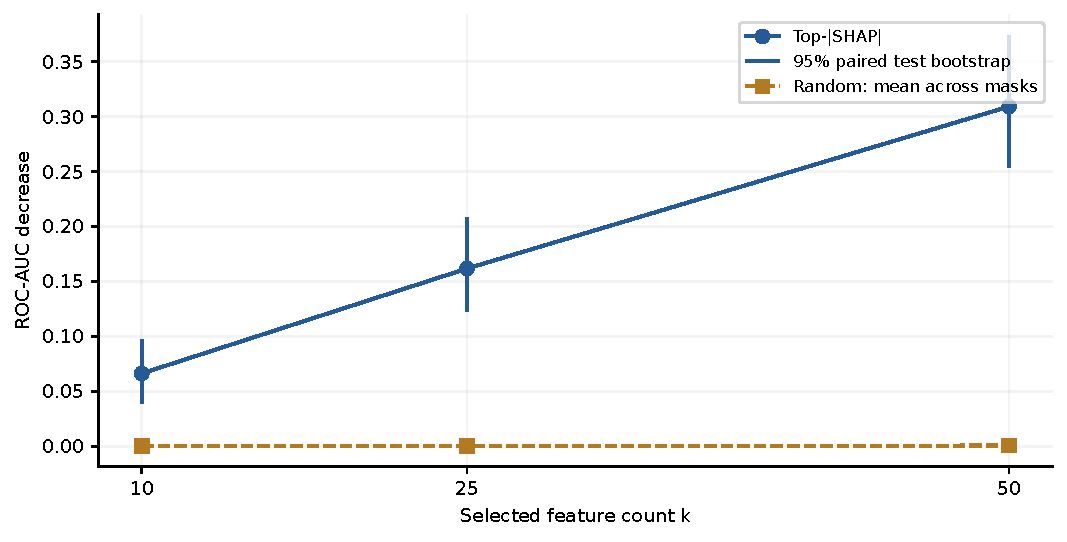
\includegraphics[width=\linewidth]{fidelity_deletion.pdf}
\caption{AUC under top-$|\mathrm{SHAP}|$ and random feature-space deletion. The
random control uses the same selected coordinate count.}
\label{fig:deletion}
\end{figure}

The explanation-geometry measures were EC=0.304373 and CF=0.587352. EC indicates
a modest positive association between pairwise similarity in standardized input
space and pairwise similarity in signed attribution space. It should not be read
as robustness to Gaussian noise or as a p-value based on 79,800 independent
pairs. CF indicates separation between positive- and negative-label SHAP
centroids relative to the largest per-sample attribution norm. It describes the
geometry of this fitted model and test set, not a causal boundary between malware
families.

Figure~\ref{fig:local-shap} provides a traceable local example from the fidelity
test set. Its role is illustrative: the aggregate conclusions come from all 400
test rows and controlled masks, not from selecting one visually persuasive case.

\begin{figure}[t]
\centering
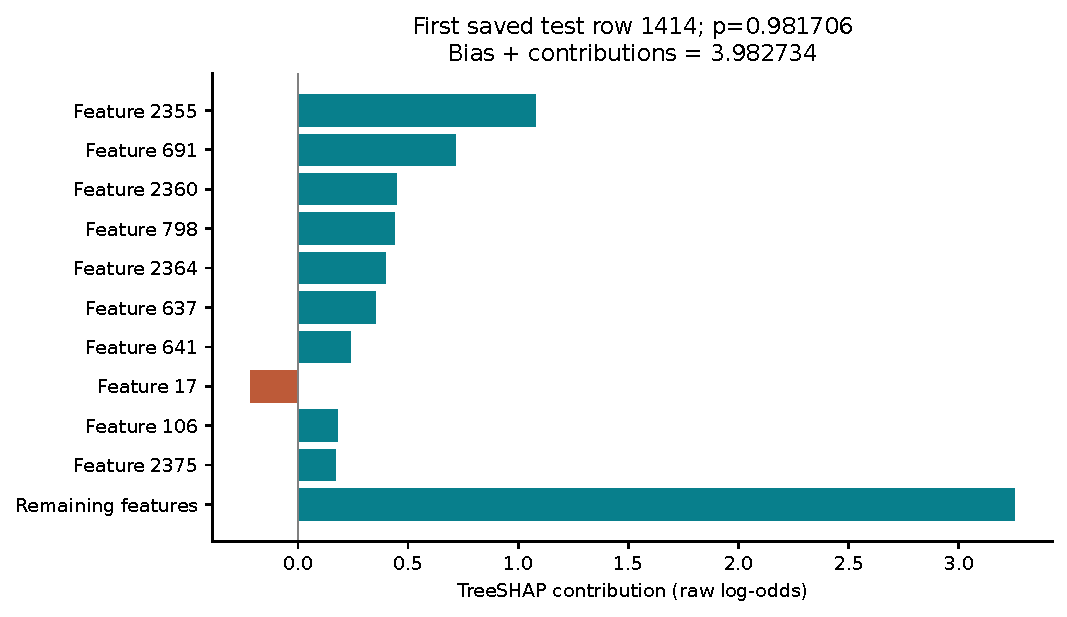
\includegraphics[width=\linewidth]{local_shap_example.pdf}
\caption{Traceable local TreeSHAP example generated from the fixed fidelity
model. Numeric coordinate labels reflect the available feature table.}
\label{fig:local-shap}
\end{figure}

RQ2 is therefore supported in a precise, limited sense: under replacement by
training-column means, coordinates ranked by absolute TreeSHAP have substantially
greater influence on the fitted model's ranking than uniformly selected
coordinates. The result does not establish that a masked vector corresponds to a
valid executable, that SHAP identifies causal ransomware behavior, or that the
same values hold for another trained model.

\subsection{RQ3: Status of PID Fusion}

The measured package records fusion as \texttt{not\_run} with the reason that real
dynamic reports aligned to validation and test IDs are required. The dynamic
template contains 800 row IDs and a schema for evidence collection, but its
provenance declares \texttt{signal\_origin=not\_collected}; it is not a result. No
synthetic score was substituted.

Consequently, this paper reports no PID AUC, AP, FPR, TPR, or latency. Values in
earlier thesis drafts cannot be traced to paired predictions under the locked
protocol and are excluded. This negative status is itself relevant to RQ3: a
valid claim requires the data lineage, ablations, state policy, and latency scope
specified in Sections~\ref{sec:problem}--\ref{sec:exp}. Until those inputs exist,
the framework contribution is the controller and evaluation design, not a
demonstrated improvement of the multi-stage system.

\section{Discussion}
\label{sec:discussion}

\subsection{Why Explanation Signals Can Complement Uncertainty}

The active-learning result suggests that output ambiguity and explanation
geometry capture related but non-identical information. Predictive uncertainty
depends on one scalar. Directional entropy distinguishes one-sided support from
strong opposing contributions, while SHAP variance distinguishes diffuse from
concentrated attributions. Their usefulness is plausible in a PE setting where
benign-looking structural metadata may coexist with suspicious imports, sections,
or byte patterns. Two samples near $p=0.5$ need not be equally informative if one
contains little evidence and the other contains a conflict among large effects.

The ablation results also caution against assigning each signal an unconditional
benefit. $U+H$ had a favorable mean FPR but lower TPR and AUC than $\xfull$;
$U+V$ had relatively strong AP but unstable FPR. The full weighted score performed
best on mean AUC and AP, yet the weights were evaluated on one local dataset and
were not optimized through an independent outer validation study. A larger study
should compare fixed preregistered weights, validation-only tuning, rank
aggregation, and diversity-aware batch selection. It should also test whether
acquisition becomes redundant when many high-scoring pool samples are near
duplicates.

The current result demonstrates ranking improvement at equal training-label
counts. It does not demonstrate label savings, because a target validation
performance was not declared before the run, and it does not demonstrate labor
savings, because expert annotation was simulated by label revelation. A
deployment study would measure time per label, adjudication, abstention, and
mislabeling, ideally with multiple analysts.

\subsection{What the Fidelity Experiment Establishes}

The deletion control answers a model-behavior question: if the coordinates that
TreeSHAP ranks highest are replaced by a training statistic, does predictive
ranking degrade more than under random replacement? Across all three budgets the
answer is yes, and the effect grows with $k$. The random baseline is essential.
Without it, an AUC decrease could be attributed merely to modifying input
coordinates. The small random drops show that the same nominal number of
uniformly selected coordinates usually has little effect on this model.

The experiment does not establish executable-level fidelity. A PE representation
contains dependent quantities: sizes, offsets, counts, hashes, and directory
metadata may obey structural constraints. Coordinate-wise mean replacement can
violate those constraints or create a vector far from the data manifold. Even
equal $k$ does not ensure equal perturbation magnitude; some selected values may
already equal their means, while a top-SHAP coordinate may be far from baseline.
The artifact records the actual number of changed coordinates and probability
change, but a stronger protocol would mask semantically coupled groups, quantify
out-of-distribution distance, and where possible reconstruct and validate a PE
file.

The approximately 630-fold ratio at $k=25$ should not be marketed as a universal
improvement factor. It divides by a random-control mean close to zero and can vary
substantially with baseline, $k$, model, split, and random seed. The more stable
statement is that the absolute top-SHAP AUC drop (0.1616) is materially larger
than the random mean (0.000257) under the frozen protocol, with a conditional
paired-bootstrap interval [0.1222, 0.2078].

EC and CF add geometric context but do not certify an explanation. EC depends on
the chosen feature standardization, cosine similarity, and Pearson comparison.
CF uses test labels and is sensitive to centroid structure and outliers. Because
FF, EC, and CF measure different constructs and do not naturally share a bounded
scale, an aggregate OFS would require a preregistered normalization, justified
weights, sensitivity analysis, and ideally correlation with external expert or
task outcomes. Reporting the components separately is scientifically stronger
than selecting a convenient weighted average after observing them.

\subsection{Role of PID in the Multi-Stage System}

The PID proposal is motivated by sequential disagreement, but its value cannot be
inferred from the controller form. A fixed average may be difficult to beat if
the two sources are stable and calibrated. A proportional rule may be sufficient
if sessions are short. Integral state can accumulate bias, and a derivative term
can amplify noisy score changes. These possibilities make P/PI/PID ablations
necessary rather than ceremonial.

A proper dynamic study must distinguish the value of the source from the value
of fusion. Static-only versus Dynamic-only quantifies individual ranking; Average
and validation-selected Fixed establish simple fusion baselines; P, PI, and PID
test whether state and temporal change contribute. The same paired inputs must be
used for every rule. If PID does not improve the baselines, the correct outcome
is to report that result and prefer the simpler model.

The claim about ``sleep evasion'' also requires care. PID cannot create behavior
that a sandbox never observes. A longer or adaptive observation policy may expose
delayed behavior; the controller can only reweight scores after dynamic evidence
arrives. Likewise, sub-millisecond arithmetic replay is not evidence of a
15-ms end-to-end decision if process startup and observation take seconds. A
future latency table should separately report static extraction, static inference,
queueing, environment startup, dynamic observation, dynamic scoring, fusion, and
end-to-end time, including median and tail quantiles.

\subsection{Operational Implications}

The framework is best understood as an allocation system. Static analysis
provides broad, early coverage. A gate allocates expensive observation to selected
cases. Active learning allocates expert labels to selected training samples.
Fidelity testing allocates trust by requiring explanations to pass controlled
behavioral checks. These allocation decisions operate at different time scales
and should have independent service-level metrics.

For a security operations center, the most immediate verified use is model
maintenance: rank uncertain pool items using $\xfull$, present the selected PE
records and evidence to analysts, and retain the queries and subsequent model
versions. The fidelity protocol can serve as a release-time diagnostic for each
candidate model. The dynamic/PID path should remain disabled as a performance
claim until collection and validation gates pass; a software implementation can
exist before its operational efficacy has been established.

Reproducibility artifacts support audit and incident review. A model checkpoint,
query list, split manifest, prediction table, and hash make it possible to answer
why a reported metric changed. They do not replace governance requirements such
as sample-handling authorization, privacy controls, malware containment, or
documented label definitions. High-quality operational evidence combines both
computational traceability and trustworthy data lineage.

\section{Threats to Validity}
\label{sec:threats}

\subsection{Construct Validity}

The largest construct threat is the relationship between the available binary
label and the stated ransomware domain. The repository does not include original
file identities or a label-definition document proving that every positive row
is ransomware. Calling the measured task ransomware detection would therefore
overstate what the data establish. We describe it as binary classification of a
local PE-feature table and treat ransomware as the motivating application.

The acquisition signals also require precise interpretation. $H$ is entropy of
positive versus negative SHAP mass, not predictive class entropy. $V$ is variance
over signed coordinates for one explanation, not uncertainty across trees or
models. The labels ``directional conflict'' and ``dispersion'' are used to avoid
claiming that either quantity is a calibrated epistemic uncertainty measure.

Fidelity is similarly multi-dimensional. A large deletion effect supports the
relationship between a ranking and fitted-model behavior under a defined
intervention. It does not prove causality, human usefulness, stability under all
perturbations, or semantic correctness. EC and CF are implementation-specific
geometric statistics. We avoid collapsing them into OFS because a composite
would obscure rather than solve these construct differences.

\subsection{Internal Validity}

The fixed row split prevents direct overlap among train, validation, and test
indices, and the audit found no exact duplicate feature vectors. It does not rule
out near-duplicates, related binaries, or shared acquisition sources across
partitions. Such dependence could inflate performance. Family-, source-, or
time-aware splitting cannot be performed without metadata.

Active-learning methods share initial sets within seeds, budgets, hyperparameters,
and test data. This controls important confounders, but fixed acquisition weights
were not selected in an independent outer loop. The policy comparison may depend
on those choices. The oracle uses existing labels and has no annotation error;
real analysts could change both selected-label quality and measured cost.

The fidelity model is trained separately from the active-learning models. This
is intentional for a fixed-model diagnostic, but it prevents a claim that the AL
improvement caused the fidelity outcome. Training means are calculated only from
the training partition, which avoids test leakage. Nonetheless, mean replacement
can induce out-of-distribution vectors, and top-SHAP versus random masks may have
different numeric magnitudes despite equal selected-coordinate counts.

No internal-validity claim is made for PID performance. The runner rejects
missing, simulated, or untraceable dynamic evidence, and the default experiment
did not execute fusion. This avoids one confound---constructing $\pdynamic$ from
the target label---but leaves RQ3 empirically unanswered.

\subsection{Statistical Conclusion Validity}

Five active-learning seeds share one test set. Their sample SD quantifies
sensitivity to initial labels and query sequences, not uncertainty over the
population of possible malware samples. Paired seed differences are appropriate
for the controlled comparison, but five pairs provide limited power and do not
justify strong distributional assumptions. We report all paired signs and avoid
a fragile significance claim.

FPR comparisons depend on thresholds selected from validation at a target TPR.
Because achieved test TPR varies, a lower FPR is not automatically a uniformly
better detector. Both rates are reported. AP is calculated from ranked
predictions using the standard step-wise definition and is not interchangeable
with trapezoidal PR area \cite{saito2015precision}.

The fidelity bootstrap resamples test rows while retaining paired original and
masked scores. Its interval is conditional on one trained model. Twenty random
masks characterize mask variability for that model and test set, not training or
dataset variability. EC uses 79,800 pairwise entries, but these entries share 400
samples, so they cannot be treated as independent observations for a conventional
Pearson test.

\subsection{External Validity}

The pilot is small relative to contemporary malware corpora and has no verified
upstream provenance. Results may change across collection periods, organizations,
malware families, benign software distributions, packers, and feature-extractor
versions. The study is neither a temporal holdout nor a family holdout, and it
does not establish zero-day performance. External validation should use a
manifested dataset with file hashes, collection dates, family/source metadata,
licensing, and independently documented labels.

The models use EMBER-style static coordinates and LightGBM. The acquisition
signals can be calculated for other additive explanations, but their behavior and
cost may differ for raw-byte networks, graph models, or sequence models. Likewise,
mean masking is not directly transferable to categorical, sparse, or structured
representations without a domain-specific baseline.

\subsection{Operational and Reproducibility Validity}

Recorded timings were obtained in a small, deterministic two-thread experiment.
They exclude several deployment costs and cannot establish endpoint throughput or
SOC response time. No real sandbox trace is included, so the work does not show
resistance to sleep evasion or environmental checks.

The evidence package provides hashes, versions, configurations, checkpoints,
queries, predictions, masks, and successful replay counts. This supports
computational reproducibility for the retained run. The compact review package
does not commit all large checkpoints and per-sample artifacts; a fresh full run
is required to regenerate them. Moreover, source and output hashes verify file
identity rather than the truth of external metadata. Reproducibility and data
authenticity are related but distinct properties.

\section{Conclusion and Future Work}
\label{sec:conclusion}

This paper presented a multi-stage framework for PE malware detection that
connects evidence fusion, explanation-guided model adaptation, and quantitative
explanation evaluation. The framework uses a LightGBM static classifier and
native TreeSHAP, defines a stateful PID rule for aligned static--dynamic scores,
selects active-learning queries through predictive uncertainty, directional
entropy, and signed SHAP variance, and tests feature rankings with controlled
deletion and equal-budget random masks.

The verified evidence supports two conclusions within a row-disjoint internal
pilot. First, the full acquisition policy improved ranking at a fixed 700-label
training budget: mean ROC--AUC was 0.9749, compared with 0.9691 for uncertainty
sampling and 0.9634 for random selection. The full policy exceeded uncertainty
sampling in AUC for all five paired seeds. Its FPR was lower in only two seeds,
so the result does not establish stable false-positive reduction. Second,
top-$|\mathrm{SHAP}|$ deletion affected the fixed fidelity model much more than
random deletion. At $k=25$, AUC fell from 0.9802 to 0.8185, while random masks
retained mean AUC 0.9799. This supports the relevance of the SHAP ranking to model
behavior under training-mean replacement, not causal or executable-level
validity.

The paper makes no empirical PID performance claim. The repository lacks real
dynamic observations aligned to the static validation/test rows, and fusion
replay time would not measure the cost of acquiring such observations. The
controller, validation grid, state policy, baselines, and factorial evaluation
are specified so that a subsequent experiment can test rather than assume its
benefit.

Three priorities govern future work. First, a dataset manifest must establish
file identities, collection time, source, family, license, and label semantics;
this enables temporal, family-held-out, and external validation. Second, dynamic
reports should be collected under a locked observation policy and paired to the
static rows, followed by Static/Dynamic/Average/Fixed/P/PI/PID ablations and
separate latency decomposition. Third, fidelity evaluation should move from
coordinate-wise means toward schema-aware group interventions, manifold checks,
and, where possible, functionality-preserving PE transformations. Further work
should also compare diversity-aware acquisition, multiple fitted fidelity models,
analyst annotation cost, and robustness to poisoning or explanation manipulation.

The broader methodological lesson is that a multi-stage security system should
not be validated by one headline AUC. Its classifier, acquisition policy,
explanations, evidence fusion, and operational timing answer different questions.
Keeping those claims separate---and attaching each to replayable evidence---is a
necessary condition for credible progress from a thesis prototype toward a
deployable detection workflow.


\appendices
\section{Acquisition Procedure}
\label{app:acquisition}

For reproducibility, the active-learning loop can be expressed without relying
on implementation-specific classes:

\begin{enumerate}
    \item Split the audited row IDs once into training/pool, validation, and test.
    For each seed, draw a stratified initial labeled subset from the training
    indices and give every acquisition policy the same subset.
    \item At round $r$, fit a new LightGBM booster on $\mathcal{L}_r$. Save the
    model before using it for acquisition.
    \item Predict validation data, select a threshold for the target validation
    TPR, and save validation and test predictions. Do not expose test metrics to
    the selection procedure.
    \item If the budget is not exhausted, predict the remaining pool. For
    explanation-based strategies, compute native TreeSHAP and verify
    (\ref{eq:additivity}). Compute and pool-normalize $U$, $H$, and $V$.
    \item Rank the pool by (\ref{eq:query}); break score ties using ascending
    original row ID. Query exactly 100 distinct rows and reveal their existing
    labels. Save scores, component signals, ranks, IDs, and labels.
    \item Move queried rows from $\mathcal{U}_r$ to $\mathcal{L}_{r+1}$ and
    repeat through round five.
\end{enumerate}

Every method begins round zero with the same predictions within a seed. The
verifier checks this equality, ensures queried IDs belong to the current pool,
and confirms that no validation/test index is added to training.

\section{Fidelity Replay Procedure}
\label{app:fidelity}

The fidelity replay uses artifacts that are independent of plot-generation code:

\begin{enumerate}
    \item Reload the saved model and the fixed training/validation/test indices.
    Recompute the training-column mean and standard deviation and compare them
    with the retained baseline archive.
    \item Predict the original test matrix and recompute native TreeSHAP. Check
    shapes, finite values, and raw-score additivity.
    \item For every retained mask, copy the original test matrix and replace
    exactly the saved per-row indices by the matching training means.
    \item Recompute masked probabilities and verify them against saved
    predictions. Recompute AUC, probability-change metrics, and actual changed
    coordinate counts.
    \item Recompute standardized feature cosine similarities, SHAP cosine
    similarities, label-conditioned centroids, EC, and CF.
    \item Confirm that no aggregate OFS appears in the summary.
\end{enumerate}

This procedure makes the numerical conclusions reproducible from a model, split,
baseline, and masks. It does not make the masked vector a valid executable and
does not recover absent upstream sample metadata.

\section{Metric and Evidence Definitions}

\begin{table*}[h]
\centering
\caption{Interpretation boundaries for reported quantities.}
\label{tab:metric-boundaries}
\small
\begin{tabular}{p{2cm}p{5.2cm}p{7.6cm}}
\toprule
Quantity & What it measures & What it does not establish \\
\midrule
ROC--AUC & Pairwise ranking of positive above negative rows & Calibration, selected operating cost, temporal/family generalization \\
AP & Precision summarized over recall thresholds & Analyst cost or a fixed-alert operating point \\
FPR/TPR & Test behavior at a validation-selected threshold & Uniform dominance when achieved TPR differs \\
Seed SD & Sensitivity to initial labels and query sequence & Population confidence interval over independent test corpora \\
$H$ & Balance of positive/negative signed SHAP mass & Predictive entropy or causal conflict \\
$V$ & Variance across coordinates of one SHAP vector & Ensemble, posterior, or across-tree uncertainty \\
Top-k AUC drop & Fixed-model sensitivity to training-mean replacement & A valid PE edit or causal ransomware behavior \\
FF & Relative probability change under a mask & A bounded percentage or universal fidelity scale \\
EC & Correlation of input/explanation pairwise geometry & Noise robustness, independence of pairs, human usefulness \\
CF & Separation of label-conditioned SHAP centroids & Causality or prospective classification performance \\
Fusion replay time & Arithmetic/controller runtime after scores exist & Sandbox, collection, model, queue, or end-to-end latency \\
SHA-256 & Identity of an input or artifact & Authenticity of its stated origin or label semantics \\
\bottomrule
\end{tabular}
\end{table*}

\section{Claim--Evidence Map}

\begin{table*}[h]
\centering
\caption{Claim--evidence map for the current manuscript.}
\label{tab:claim-evidence}
\scriptsize
\setlength{\tabcolsep}{3pt}
\begin{tabular}{p{4.9cm}p{4.5cm}p{1.8cm}p{3.0cm}}
\toprule
Claim & Primary evidence & Status & Scope \\
\midrule
$\xfull$ has higher final AUC than uncertainty sampling & \texttt{al/summary.json}, paired differences, final checkpoints & Verified & Five paired seeds; shared row-disjoint test \\
$\xfull$ always lowers FPR & Paired FPR differences & Rejected & Lower in only 2/5 seeds \\
Top-SHAP deletion changes predictions more than random deletion & Fidelity masks, predictions, deletion summary & Verified & One fixed model; training-mean feature-space masks \\
SHAP values reconstruct raw LightGBM outputs & Saved contribution matrices and verifier & Verified & Numeric additivity, not semantic correctness \\
EC=0.304373 and CF=0.587352 & Replayed similarity/centroid inputs & Verified & Geometry of one test/model \\
OFS certifies explanation quality & No validated aggregation rule & Not supported & Components reported separately \\
PID improves AUC/FPR or sleep-evasion resistance & Dynamic template has no observed scores & Not measured & Method/protocol only \\
Fusion latency is end-to-end system latency & Replay scope excludes collection/inference/I/O & Not supported & Requires separate measurement \\
Results demonstrate ransomware family/zero-day detection & Original identities/families/times absent & Not supported & Binary local pilot only \\
\bottomrule
\end{tabular}
\end{table*}

\section{Reproducibility Checklist}

The current evidence package records the following items:

\begin{itemize}
    \item exact input CSV SHA-256, row and feature counts, class counts, split
    indices, and exact-duplicate-vector audit;
    \item repository commit, clean working-tree status at run time, Python and
    library versions, model hyperparameters, seeds, thread count, query weights,
    tie policy, and timing scope;
    \item 150 active-learning checkpoints, per-round metrics, query IDs/ranks,
    component scores, validation/test predictions, and paired differences in the
    complete run;
    \item fidelity model, training baseline, TreeSHAP vectors, mask indices,
    pre/post-mask predictions, bootstrap resamples, and geometry inputs in the
    complete run;
    \item generated Markdown, CSV, JSON, LaTeX, PDF, and PNG review artifacts,
    with a package-wide checksum list;
    \item an independent verification summary confirming replay counts for the
    selected run.
\end{itemize}

The compact repository review package omits some large model and prediction files
described by its reports. Reproduction should create a new output directory,
verify the input hash, preserve the locked configuration, and run the verifier on
the fresh output. Results from altered data or configuration should be reported as
a separate experiment rather than silently replacing the measured package.

\section{Requirements for the Pending Dynamic Study}

Before the PID subsection can be promoted from method to empirical contribution,
the following conditions must be met:

\begin{enumerate}
    \item Each validation/test \texttt{row\_id} maps to an authorized original sample and
    exactly one documented observation report with a verified content hash.
    \item The mapping from observed events to $\pdynamic$ is frozen before test
    evaluation and documented as either a calibrated probability or risk score.
    It must not read the target label or $\pstatic$.
    \item \texttt{sequence\_id} and order represent a real session. Validation and test
    sessions are disjoint, and controller state is reset at their boundaries.
    \item Static-only, Dynamic-only, Average, Fixed, P, PI, PID, and reference PID
    receive the same paired signals and test rows. All choices occur on
    validation.
    \item FPR is reported with achieved TPR; AUC and AP use saved test scores; all
    per-row fused scores and weights are retained.
    \item Timing separately records collection, feature extraction, static and
    dynamic inference, fusion, queueing, and end-to-end response. Workload,
    hardware, warm/cold state, and observation policy are reported.
    \item If interaction with active learning is claimed, the full
    Fixed/PID $\times$ Random/$\xfull$ design is evaluated and the
    difference-in-differences is reported even when it is zero or unfavorable.
\end{enumerate}

These requirements are deliberately stricter than accepting a demo trace. They
ensure that a future improvement can be attributed to the fusion rule rather than
label leakage, incomparable signals, threshold tuning on test, or an unmeasured
change in the observation process.


\bibliographystyle{IEEEtran}
\bibliography{references}

\end{document}
